
%%-----------------------------------------------------------------------------
\section{Application: Using Taylor's Theorem to Approximate Functions.}

The material for the remainder of this book was taken from Sean Mauch's 
{\bf Applied mathematics} text\footnote{It is in the public domain and available at
\url{http://www.its.caltech.edu/~sean/book.html}.}.


\begin{theorem}
{\bf Taylor's Theorem of the Mean.}
{\rm
If $f(x)$ is $n+1$ times continuously differentiable in $(a,b)$ then there
exists a point $x = \xi \in (a,b)$ such that
\begin{equation}
  \label{taylors_theorem}
  f(b) = f(a) + (b-a) f'(a) + \frac{(b-a)^2}{2!} f''(a) + \cdots + 
  \frac{(b-a)^n}{n!} f^{(n)}(a) 
  + \frac{(b-a)^{n+1}}{(n+1)!} f^{(n+1)}(\xi).
\end{equation}
For the case $n = 0$, the formula is
\[
f(b) = f(a) + (b-a) f'(\xi),
\]
which is just a rearrangement of the terms in the theorem of the mean,
\[
f'(\xi) = \frac{f(b) - f(a)}{b-a}.
\]
}
\end{theorem}
%% CONTINUE: Prove.



One can use Taylor's theorem to approximate functions with polynomials.
Consider an infinitely differentiable function $f(x)$ and a point $x = a$.  
Substituting $x$ for $b$ into Equation~\ref{taylors_theorem} we obtain,
\[
\label{taylors_theorem_x}
f(x) = f(a) + (x-a) f'(a) + \frac{(x-a)^2}{2!} f''(a) + \cdots + 
\frac{(x-a)^n}{n!} f^{(n)}(a) 
+ \frac{(x-a)^{n+1}}{(n+1)!} f^{(n+1)}(\xi).
\]
If the last term in the sum is small then we can approximate our function
with an $n^{th}$ order polynomial.
\[
f(x) \approx f(a) + (x-a) f'(a) + \frac{(x-a)^2}{2!} f''(a) + \cdots + 
\frac{(x-a)^n}{n!} f^{(n)}(a) 
\]
The last term in Equation~\ref{taylors_theorem_x} is called the remainder
or the error term,
\[
R_n = \frac{(x-a)^{n+1}}{(n+1)!} f^{(n+1)}(\xi).
\]
Since the function is infinitely differentiable, $f^{(n+1)}(\xi)$ exists and
is bounded.  Therefore we note that the error must vanish as $x \to 0$ 
because of the $(x-a)^{n+1}$ factor.  We therefore suspect that our 
approximation would be a good one if $x$ is close to $a$.  Also note that
$n!$ eventually grows faster than $(x-a)^n$,
\[
\lim_{n \to \infty} \frac{(x-a)^n}{n!} = 0.
\]
So if the derivative term, $f^{(n+1)}(\xi)$, does not grow to quickly, the
error for a certain value of $x$ will get smaller with increasing $n$ and
the polynomial will become a better approximation of the function.
(It is also possible that the derivative factor grows very quickly and 
the approximation gets worse with increasing $n$.)




\begin{example}
{\rm
  Consider the function $f(x) = e^x$.  We want a polynomial approximation of
  this function near the point $x = 0$.  Since the derivative of $e^x$ is
  $e^x$, the value of all the derivatives at $x = 0$ is $f^{(n)}(0) = e^0 = 1$.
  Taylor's theorem thus states that
  \[
  e^x = 1 + x + \frac{x^2}{2!} + \frac{x^3}{3!} + \cdots + \frac{x^n}{n!}
  + \frac{x^{n+1}}{(n+1)!} e^\xi,
  \]
  for some $\xi \in (0,x)$.  The first few polynomial approximations of 
  the exponent about the point $x = 0$ are 
  \begin{align*}
    f_1(x) &= 1 \\
    f_2(x) &= 1 + x \\
    f_3(x) &= 1 + x + \frac{x^2}{2} \\
    f_4(x) &= 1 + x + \frac{x^2}{2} + \frac{x^3}{6} 
  \end{align*}
  The four approximations are graphed in Figure~\ref{tayexp4}.

\begin{figure}[h!]
%\begin{tabular}{cc}
\begin{minipage}{\textwidth}
\begin{center}
%\vspace{1.0 cm}
%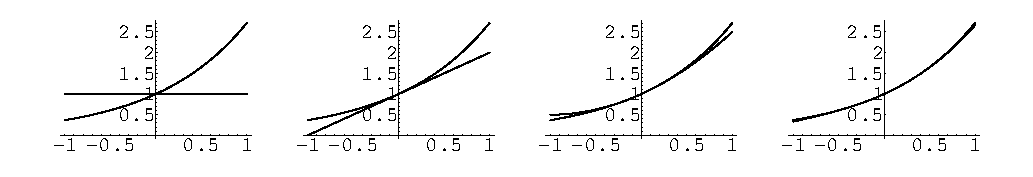
\includegraphics[height=3cm,width=8cm]{tayexp4.eps}
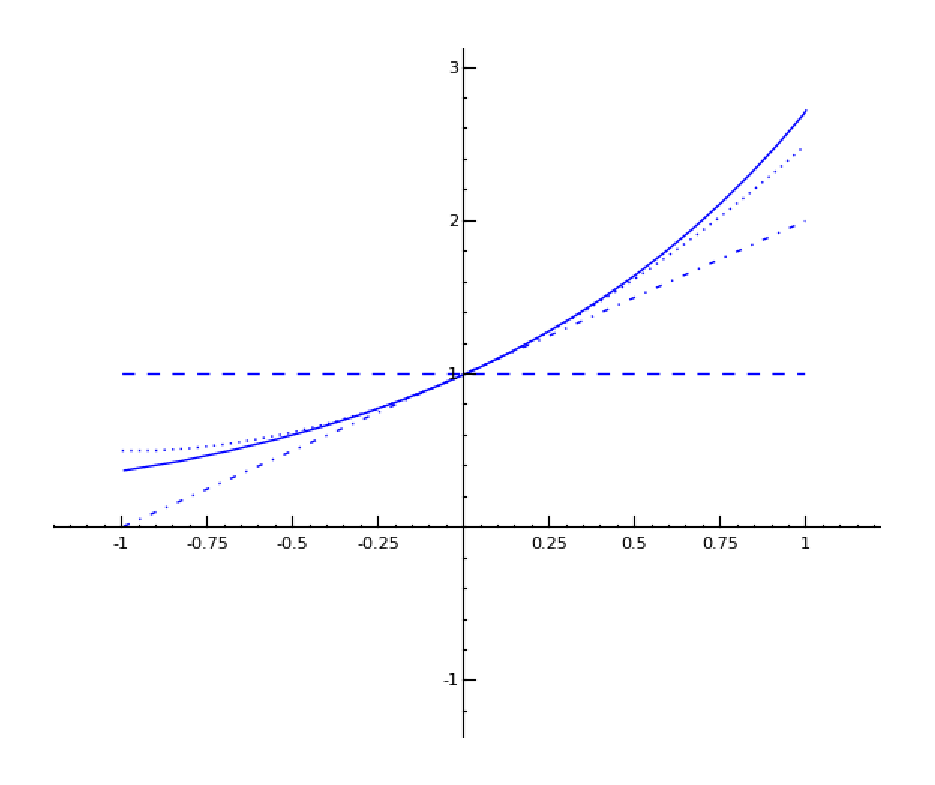
\includegraphics[height=6cm,width=8cm]{tayexp3.eps}
\end{center}
\end{minipage}
%\caption{Mauch's Four Finite Taylor Series Approximations of $e^x$.}
\caption{Finite Taylor Series Approximations of $1$, $1+x$, $1+x+\frac{x^2}{2}$ to $e^x$.}
\label{fig:tayexp4}
\label{tayexp4}
\end{figure}
%sage: p1 = plot(exp(x),-1,1)
%sage: p2 = plot(x^0,-1,1,linestyle="--")
%sage: p3 = plot(x^0+x,-1,1,linestyle="-.")
%sage: p4 = plot(x^0+x+x^2/2,-1,1,linestyle=":")
%sage: show(p1+p2+p3+p4)


  Note that for the range of $x$ we are looking at, the approximations
  become more accurate as the number of terms increases.

Here is one way to compute these approximations using \sage:


\vskip .1in

\begin{Verbatim}[fontsize=\scriptsize,fontfamily=courier,fontshape=tt,frame=single,label=\sage]

sage: x = var("x")
sage: y = exp(x)
sage: a = lambda n: diff(y,x,n)(0)/factorial(n)
sage: a(0)
1
sage: a(1)
1
sage: a(2)
1/2
sage: a(3)
1/6
sage: taylor = lambda n: sum([a(i)*x^i for i in range(n)])
sage: taylor(2)
x + 1
sage: taylor(3)
x^2/2 + x + 1
sage: taylor(4)
x^3/6 + x^2/2 + x + 1

\end{Verbatim}


}
\end{example}


\begin{example}
{\rm
  Consider the function $f(x) = \cos x$.  We want a polynomial approximation of
  this function near the point $x = 0$. The first few derivatives of $f$ are
  \begin{align*}
    f(x) &= \cos x \\
    f'(x) &= - \sin x \\
    f''(x) &= - \cos x \\
    f'''(x) &= \sin x \\
    f^{(4)}(x) &= \cos x
  \end{align*} 
  It's easy to pick out the pattern here,
  \[
  f^{(n)}(x) = 
  \begin{cases}
    (-1)^{n/2} \cos x &\text{for even } n, \\
    (-1)^{(n+1)/2} \sin x & \text{for odd } n.
  \end{cases}
  \]
  Since $\cos(0) = 1$ and $\sin(0) = 0$ the $n$-term approximation of the
  cosine is,
  \[
  \cos x = 1 - \frac{x^2}{2!} + \frac{x^4}{4!} - \frac{x^6}{6!} + \cdots
  + (-1)^{2(n-1)} \frac{x^{2(n-1)}}{(2(n-1))!} 
  + \frac{x^{2n}}{(2n)!} \cos \xi.
  \]
  Here are graphs of the one, two, three and four term approximations.

\begin{figure}[h!]
%\begin{tabular}{cc}
\begin{minipage}{\textwidth}
\begin{center}
%\vspace{1.0 cm}
%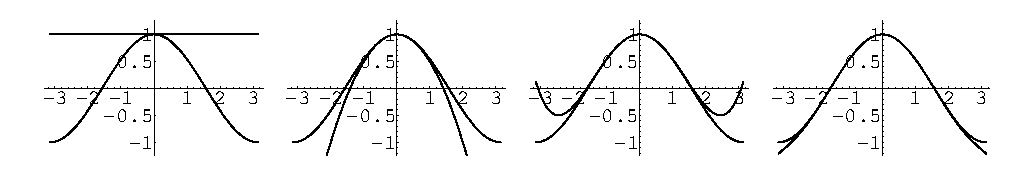
\includegraphics[height=4cm,width=7cm]{taycos4.eps}
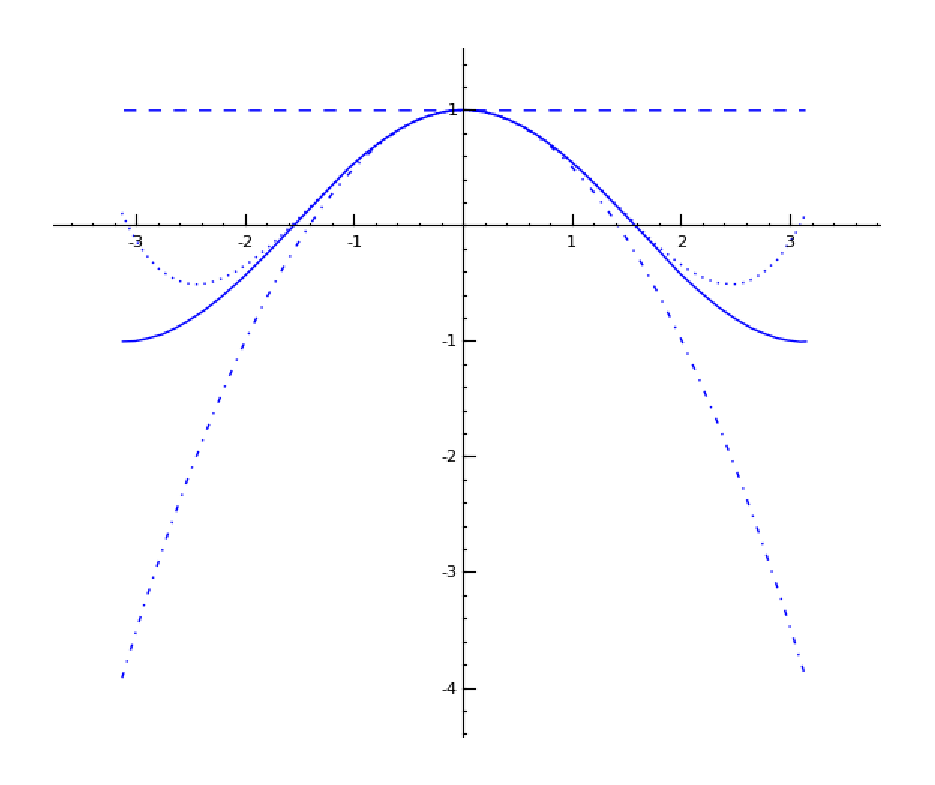
\includegraphics[height=4cm,width=7cm]{taycos3.eps}
\end{center}
\end{minipage}
%\caption{Mauch's Taylor Series Approximations of $\cos x$.}
\caption{Taylor Series Approximations of $1$, $1-\frac{x^2}{2}$, $1-\frac{x^2}{2}+\frac{x^4}{4!}$ to $\cos x$.}
\label{fig:taycos4}
\label{taycos4}
\end{figure}
%sage: p1 = plot(cos(x),-pi,pi)
%sage: p2 = plot(x^0,-pi,pi,linestyle="--")
%sage: p3 = plot(x^0-x^2/2,-pi,pi,linestyle="-.")
%sage: p4 = plot(x^0-x^2/2+x^4/24,-pi,pi,linestyle=":")
%sage: show(p1+p2+p3+p4)
%sage: p1 = plot(cos(x),-2*pi,2*pi)
%sage: p4 = plot(x^0-x^2/2+x^4/24-x^6/720+x^8/40320,-2*pi,2*pi,linestyle=":")
%sage: show(p1+p4)

  Note that for the range of $x$ we are looking at, the approximations
  become more accurate as the number of terms increases.
  Consider the ten term approximation of the cosine about $x = 0$,
  \[
  \cos x = 1 - \frac{x^2}{2!} + \frac{x^4}{4!} - \cdots - \frac{x^{18}}{18!} 
  + \frac{x^{20}}{20!} \cos \xi.
  \]
  Note that for any value of $\xi$, $|\cos \xi| \leq 1$.  Therefore the absolute
  value of the error term satisfies,
  \[
  | R | = \left| \frac{x^{20}}{20!} \cos \xi \right| \leq \frac{|x|^{20}}{20!}.
  \]

%$x^{20}/20!$ is plotted in Figure~\ref{taycoser}.
%\begin{figure}[h!]
%\begin{tabular}{cc}
%\begin{minipage}{\textwidth}
%\begin{center}
%\vspace{1.0 cm}
%\includegraphics[height=4cm,width=7cm]{taycoser.eps}
%\end{center}
%\end{minipage}
%\caption{Mauch's Plot of $x^{20}/20!$.}
%\label{fig:taycoser}
%\label{taycoser}
%\end{figure}


  Note that the error is very small for $x < 6$, fairly small but non-negligible
  for $x \approx 7$ and large for $x > 8$.  The ten term approximation of
  the cosine, plotted below, behaves just we would predict.

\begin{figure}[h!]
%\begin{tabular}{cc}
\begin{minipage}{\textwidth}
\begin{center}
%\vspace{1.0 cm}
%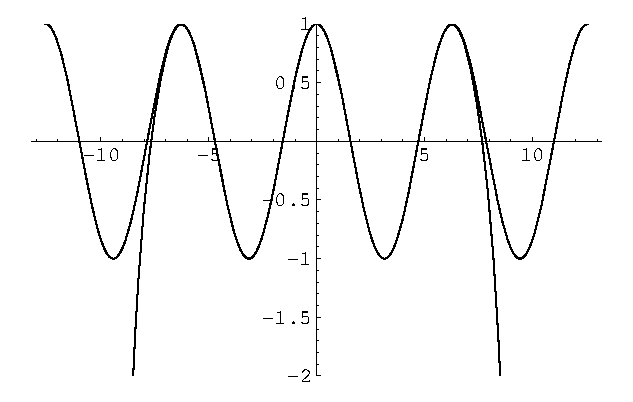
\includegraphics[height=4cm,width=7cm]{taycos10.eps}
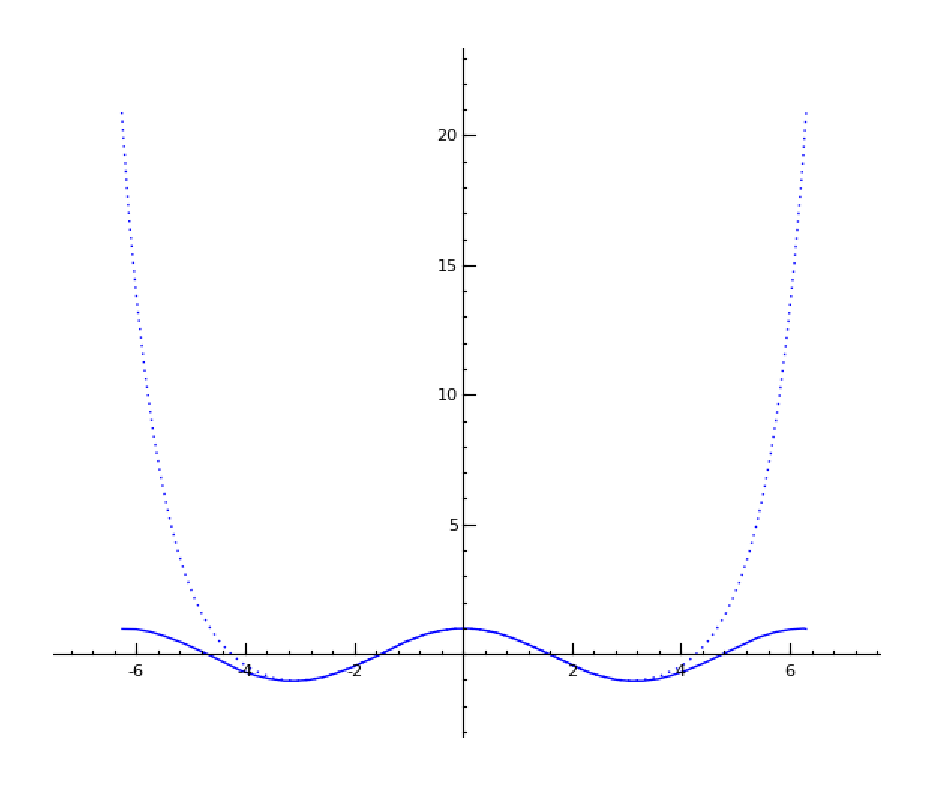
\includegraphics[height=4cm,width=7cm]{taycos10b.eps}
\end{center}
\end{minipage}
%\caption{Mauch's Ten Term Taylor Series Approximation of $\cos x$.}
\caption{Taylor Series Approximation of $1-\frac{x^2}{2}+\frac{x^4}{4!}-\frac{x^6}{6!}+\frac{x^8}{8!}$ to $\cos x$.}
\label{fig:taycos10}
\label{taycos10}
\end{figure}


  The error is very small until it becomes non-negligible at $x \approx 7$
  and large at $x \approx 8$.
}
\end{example}


\begin{example}
{\rm
  Consider the function $f(x) = \ln x$.  We want a polynomial approximation of
  this function near the point $x = 1$. The first few derivatives of $f$ are
  \begin{align*}
    f(x) &= \ln x \\
    f'(x) &= \frac{1}{x} \\
    f''(x) &= - \frac{1}{x^2} \\
    f'''(x) &= \frac{2}{x^3} \\
    f^{(4)}(x) &= - \frac{3}{x^4}
  \end{align*}
  The derivatives evaluated at $x = 1$ are
  \[
  f(1) = 0, \qquad f^{(n)}(1) = (-1)^{n-1} (n-1)!,\ \ \ \text{ for } n \geq 1.
  \]
  By Taylor's theorem of the mean we have,
  \[
  \ln x = (x-1) - \frac{(x-1)^2}{2} + \frac{(x-1)^3}{3} - \frac{(x-1)^4}{4}
  + \cdots + (-1)^{n-1} \frac{(x-1)^n}{n} 
  + (-1)^n \frac{(x-1)^{n+1}}{n+1} \frac{1}{\xi^{n+1}}.
  \]
  Below are plots of the 1, 2, and 3 term approximations.  

\begin{figure}[h!]
%\begin{tabular}{cc}
\begin{minipage}{\textwidth}
\begin{center}
%\vspace{1.0 cm}
%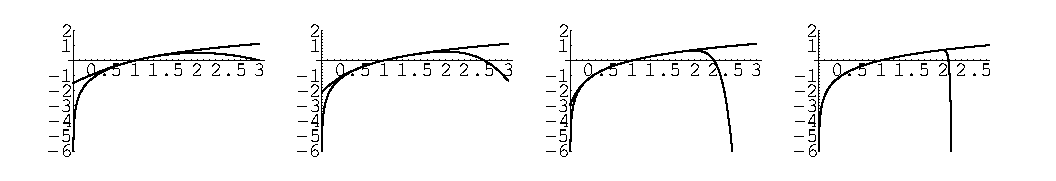
\includegraphics[height=3cm,width=10cm]{taylnt4.eps}
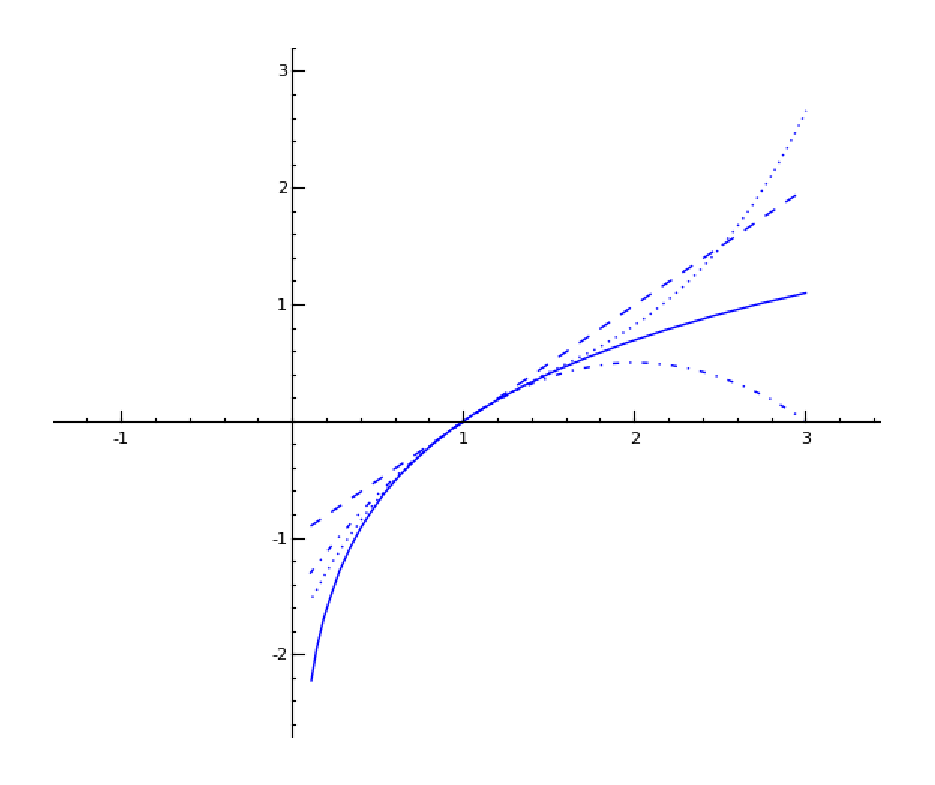
\includegraphics[height=6cm,width=10cm]{taylnt3.eps}
\end{center}
\end{minipage}
%\caption{Mauch's The 2, 4, 10 and 50 Term Approximations of $\ln x$.}
\caption{Taylor series (about $x=1$) approximations of $x-1$, $x-1-\frac{(x-1)^2}{2}$,
$x-1-\frac{(x-1)^2}{2}+\frac{(x-1)^3}{3}$ to $\ln x$.}
\label{fig:taylnt4}
\label{taylnt4}
\end{figure}


  Note that the 
  approximation gets better on the interval $(0,2)$ and worse outside this
  interval as the number of terms increases.  The Taylor series converges to
  $\ln x$ only on this interval.
}
\end{example}





%%-----------------------------------------------------------------------------
\section{Example/Application: Finite Difference Schemes}
%% Written by Saun Mauch


\begin{example}
Suppose you sample a function at the discrete points $n \Delta x$, 
$n \in \zzz$.  In Figure~\ref{sindata} we sample the function 
$f(x) = \sin x$ on the interval $[-4,4]$ with $\Delta x = 1/4$ and 
plot the data points.  

\begin{figure}[h!]
%\begin{tabular}{cc}
\begin{minipage}{\textwidth}
\begin{center}
%\vspace{1.0 cm}
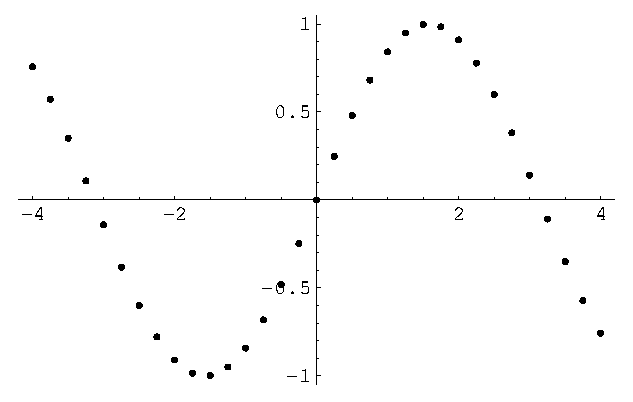
\includegraphics[height=4cm,width=7cm]{sindata.eps}
\end{center}
\end{minipage}
\caption{Sine function sampling.} % Mauch's
\label{fig:sindata}
\label{sindata}
\end{figure}


We wish to approximate the derivative of the function on the grid points
using only the value of the function on those discrete points.  From
the definition of the derivative, one is lead to the formula

  \begin{equation}
    \label{first_order_scheme}
    f'(x) \approx \frac{f(x+\Delta x) - f(x)}{\Delta x}.
  \end{equation}

Taylor's theorem states that
  \[
  f(x + \Delta x) = f(x) + \Delta x f'(x) + \frac{\Delta x^2}{2} f''(\xi).
  \]
Substituting this expression into our formula for approximating the derivative
we obtain

  \[
  \frac{f(x+\Delta x) - f(x)}{\Delta x} = \frac{f(x) + \Delta x f'(x)
    + \frac{\Delta x^2}{2} f''(\xi) - f(x) }{\Delta x}
  = f'(x) + \frac{\Delta x}{2} f''(\xi).
  \]
Thus we see that the error in our approximation of the first derivative is
$\frac{\Delta x}{2} f''(\xi)$.  Since the error has a linear factor of 
$\Delta x$, we call this a first order accurate method.  Equation
~\ref{first_order_scheme} is called the 
\textit{forward difference scheme} for calculating the 
first derivative.  Figure~\ref{fwdsin} shows 
a plot of the value of this scheme for the function $f(x) = \sin x$ and 
$\Delta x = 1/4$.  The first derivative of the function $f'(x) = \cos x$ 
is shown for comparison.

 
\begin{figure}[h!]
%\begin{tabular}{cc}
\begin{minipage}{\textwidth}
\begin{center}
%\vspace{1.0 cm}
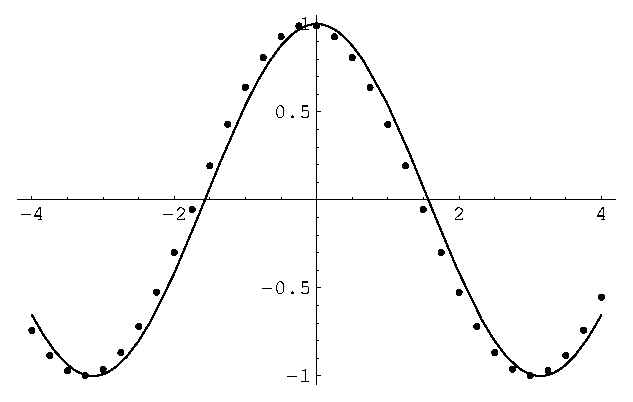
\includegraphics[height=4cm,width=7cm]{fwdsin.eps}
\end{center}
\end{minipage}
\caption{Forward Difference Scheme Approximation of the Derivative.} %Mauch's
\label{fig:fwdsin}
\label{fwdsin}
\end{figure}


Another scheme for approximating the first derivative is the 
\textit{centered difference scheme},

\[
  f'(x) \approx \frac{f(x+\Delta x) - f(x-\Delta x)}{2 \Delta x}.
\]
Expanding the numerator using Taylor's theorem,

\begin{align*}
    &\frac{f(x+\Delta x) - f(x-\Delta x)}{2 \Delta x} \\
    &\qquad= \frac{f(x) + \Delta x f'(x) + \frac{\Delta x^2}{2} f''(x)
      + \frac{\Delta x^3}{6} f'''(\xi)
      - f(x) + \Delta x f'(x) - \frac{\Delta x^2}{2} f''(x)
      + \frac{\Delta x^3}{6} f'''(\psi) }{2 \Delta x} \\
    &\qquad= f'(x) + \frac{\Delta x^2}{12}(f'''(\xi) + f'''(\psi)).
\end{align*}
The error in the approximation is quadratic in $\Delta x$.  Therefore
this is a second order accurate scheme.
Below is a plot of the derivative of the function and the 
value of this scheme for the function $f(x) = \sin x$ and $\Delta x = 1/4$.

\begin{figure}[h!]
%\begin{tabular}{cc}
\begin{minipage}{\textwidth}
\begin{center}
%\vspace{1.0 cm}
\includegraphics[height=4cm,width=7cm]{ctrsin.eps}
\end{center}
\end{minipage}
\caption{Centered Difference Scheme Approximation of the Derivative.} %Mauch's
\label{fig:ctrsin}
\label{ctrsin}
\end{figure}

Notice how the centered difference scheme gives a better approximation of the 
derivative than the forward difference scheme.
\end{example}





